\documentclass{beamer}
\mode<presentation>


\usepackage[brazil]{babel}
\usepackage[utf8]{inputenc}
 


\usepackage{amsfonts}
\usepackage{amssymb}
\usepackage{amsmath}
\usepackage{algorithm}
\usepackage{algpseudocode}



\usepackage{ae}
\usepackage{graphicx,color}
\usepackage[all]{xy}
\usepackage{empheq}
\usepackage{fancybox}
\usepackage{textcomp}
\usepackage[all]{xy}
\usepackage{textpos}
\usepackage{multicol}
\usepackage{cancel}
\usepackage{listings}
\usepackage{xcolor}
\usepackage{enumerate}
\usepackage{minted}

\usepackage[style=verbose]{biblatex}
\addbibresource{bibtex.bib}

\usepackage{tikz}
\usetikzlibrary{positioning}
\usetikzlibrary{shapes.geometric, arrows}
\usepackage{tkz-graph}
\GraphInit[vstyle = Shade]
\tikzset{
  LabelStyle/.style = { rectangle, rounded corners, draw,
                        minimum width = 2em, fill = yellow!50,
                        text = red, font = \bfseries },
  VertexStyle/.append style = { inner sep=5pt,
                                font = \Large\bfseries},
  EdgeStyle/.append style = {->, bend left} }
\thispagestyle{empty}

\tikzstyle{startstop} = [rectangle, rounded corners, minimum width=3cm, minimum 
\tikzstyle{io} = [trapezium, trapezium left angle=70, trapezium right angle=110, minimum width=3cm, minimum height=1cm, text centered, draw=black, fill=blue!30]
\tikzstyle{process} = [rectangle, minimum width=3cm, minimum height=1cm, text centered, draw=black, fill=orange!30]
\tikzstyle{decision} = [diamond, minimum width=3cm, minimum height=1cm, text centered, draw=black, fill=green!30]
\tikzstyle{arrow} = [thick,->,>=stealth]

\newcommand{\floor}[1]{$\lfloor$ #1 $\rfloor$}

\newcommand\Fontvi{\fontsize{9}{7.2}\selectfont}



\usetheme{Boadilla}

\newcommand{\PC}[1]{\ensuremath{\left(#1\right)}}


\newcommand*{\colorboxed}{}
\def\colorboxed#1#{%
  \colorboxedAux{#1}%
}
\newcommand*{\colorboxedAux}[3]{%
  % #1: optional argument for color model
  % #2: color specification
  % #3: formula
  \begingroup
    \colorlet{cb@saved}{.}%
    \color#1{#2}%
    \boxed{%
      \color{cb@saved}%
      #3%
    }%
  \endgroup
}



\title {Pensando Computacionalmente}

\author[Wladimir Araújo Tavares]{ Wladimir Araújo Tavares$^{1}$  }

\institute[UFC]{$^{1}$Universidade Federal do Ceará - Campus de Quixadá\\}
\date{}
\AtBeginSection[]
{
  \begin{frame}<beamer>{}
    \small
    \tableofcontents[currentsection,currentsubsection]
  \end{frame}
}
\begin{document}

\begin{frame}
	\titlepage
\end{frame}

%%%%%%%%%%%%%%%%%%%%%%%%%%%%%%%%%%%%%%%%%%%%%%%%%%%%%%%%%%%%%%%%%%%%



\begin{frame}{Problema dos selos}

\begin{itemize}
\item \textbf{Objetivos:} Desenvolver o pensamento computacional.

\item \textbf{Público-alvo:}  Alunos a partir do primeiro ano do Ensino Médio.

\item \textbf{Conteúdo:} Reconhecimento de padrão, pensamento indutivo

\item \textbf{Tempo:} 50 minutos

\item \textbf{Recursos:} Papel, Caneta.

\end{itemize}
    
\end{frame}


\begin{frame}{Passo 1 - Apresentação da Atividade}

\begin{itemize}
   
\item <1-> Uma agência dos correios possui apenas selos de 3 e 5 centavos. O funcionário da agência dos correios sabe que toda carta com valor postal com valor maior ou igual a 8 centavos pode ser feita usando esses selos. Ajude o funcionário da agência a encontrar essa combinação de selos que deve ser usada para um valor postal $n \geq 8$
\end{itemize}

\end{frame}


\begin{frame}{Passo 1 - Apresentação da Atividade}

\begin{itemize}
    \item <1->Primeiramente, vamos analisar as primeiras postagem para tentar descobrir uma padrão:

    \begin{itemize}
    \item<2->  8 = 3 + 5
    \item<3->  9 = 3 + 3 + 3
    \item<4-> 10 = 5 + 5
    \item<5-> 11 = 5 + 3 + 3
    \item<6-> 12 = 3 + 3 + 3 + 3
    \item<7-> 13 = 5 + 5 + 3
\end{itemize}

   \item <8->Agora, vamos tentar encontrar um padrão que leva de um valor de postagem k para um valor de postagem k+1.  
   
   \item <9-> Note que podemos substituir um selo de 5 centavos por dois selos de 3 centavos e aumentamos em uma unidade.
   
   \item <10-> Quando não tivermos selo de 5 centavos, podemos substituir 3 selos de 3 centavos por dois selos de 5 centavos.
   
   

\end{itemize}





\end{frame}


\begin{frame}{Passo 1 - Apresentação da Atividade}

\begin{itemize}
   
\item <1-> Seja uma postagem de valor $n$ realizada por $n_a$ selos de 3 centavos e $n_b$ selos de 5 centavos.

$$n  = 3n_a + 5n_b$$


\item <2-> Se $n_b$ for maior ou igual a 1 então o próximo valor de postagem pode ser obtido removendo um selo de 5 centavos e adicionando dois selos de 3 centavos.



\item <2-> Se $n_b$ b for igual a zero então o próximo valor de postagem pode ser obtido removendo 3 selos de 3 centavos e adicionado 2 selos de 5 centavos.




\end{itemize}


\end{frame}


\begin{frame}{Passo 1 - Apresentação da Atividade}


\begin{figure}
\begin{center}
	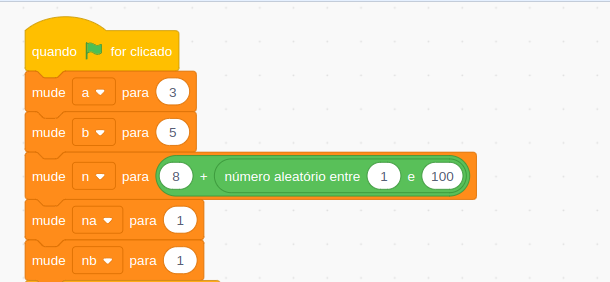
\includegraphics[scale=0.5]{images/init.png} 
\end{center}
\caption{Projeto: \url{https://scratch.mit.edu/projects/658269622/}}
\end{figure}



\end{frame}


\begin{frame}{Passo 1 - Apresentação da Atividade}


\begin{figure}
\begin{center}
	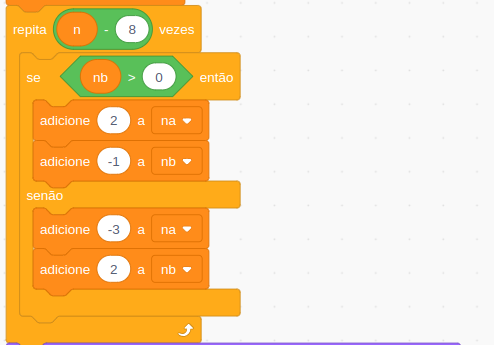
\includegraphics[scale=0.5]{images/loop.png} 
\end{center}
\caption{Projeto: \url{https://scratch.mit.edu/projects/658269622/}}
\end{figure}



\end{frame}



\begin{frame}{Passo 1 - Apresentação da Atividade}


\begin{figure}
\begin{center}
	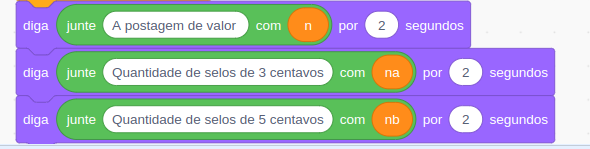
\includegraphics[scale=0.5]{images/output.png} 
\end{center}
\caption{Projeto: \url{https://scratch.mit.edu/projects/658269622/}}
\end{figure}



\end{frame}


\begin{frame}{Passo 2 - Execução}

\begin{itemize}
    \item Os valores dos selos mudaram e agora a agência de selos possui apenas 4 e 7 centavos. O funcionário da agência dos correios descobriu que toda carta com valor postal com valor maior ou igual a 18 centavos pode ser feita usando esses selos. Ajude o funcionário da agência a encontrar essa combinação de selos que deve ser usada para um valor postal $n \geq 18$. Em seguida, faça o programa que encontra essa combinação.
\end{itemize}



\end{frame}


\begin{frame}{Passo 3 - Avaliação e Discussão}

\begin{itemize}
\item<1-> Os alunos são incentivados a escrever sobre o que eles aprenderam com essa atividade.

\item<2-> Os alunos são incentivados a refletirem como os algoritmos podem nos ajudar a realizar tarefas do dia a dia. 
 
\end{itemize}




\end{frame}










\end{document}